
% ----------------------------------------------------------------------
%                   LATEX TEMPLATE FOR PhD THESIS
% ----------------------------------------------------------------------

% based on Harish Bhanderi's PhD/MPhil template, then Uni Cambridge
% http://www-h.eng.cam.ac.uk/help/tpl/textprocessing/ThesisStyle/
% corrected and extended in 2007 by Jakob Suckale, then MPI-CBG PhD programme
% and made available through OpenWetWare.org - the free biology wiki


%: Style file for Latex
% Most style definitions are in the external file PhDthesisPSnPDF.
% In this template package, it can be found in ./Latex/Classes/
\documentclass[oneside,11pt]{Latex/Classes/PhDthesisPSnPDF}


%: Macro file for Latex
% Macros help you summarise frequently repeated Latex commands.
% Here, they are placed in an external file /Latex/Macros/MacroFile1.tex
% An macro that you may use frequently is the figuremacro (see introduction.tex)
% This file contains macros that can be called up from connected TeX files
% It helps to summarise repeated code, e.g. figure insertion (see below).

% insert a centered figure with caption and description
% parameters 1:filename, 2:title, 3:description and label
\newcommand{\figuremacro}[3]{
	\begin{figure}[htbp]
		\centering
		\includegraphics[width=1\textwidth]{#1}
		\caption[#2]{\textbf{#2} - #3}
		\label{#1}
	\end{figure}
}

% insert a centered figure with caption and description AND WIDTH
% parameters 1:filename, 2:title, 3:description and label, 4: textwidth
% textwidth 1 means as text, 0.5 means half the width of the text
\newcommand{\figuremacroW}[4]{
	\begin{figure}[htbp]
		\centering
		\includegraphics[width=#4\textwidth]{#1}
		\caption[#2]{\textbf{#2} - #3}
		\label{#1}
	\end{figure}
}

% inserts a figure with wrapped around text; only suitable for NARROW figs
% o is for outside on a double paged document; others: l, r, i(inside)
% text and figure will each be half of the document width
% note: long captions often crash with adjacent content; take care
% in general: above 2 macro produce more reliable layout
\newcommand{\figuremacroN}[3]{
	\begin{wrapfigure}{o}{0.5\textwidth}
		\centering
		\includegraphics[width=0.48\textwidth]{#1}
		\caption[#2]{{\small\textbf{#2} - #3}}
		\label{#1}
	\end{wrapfigure}
}

% predefined commands by Harish
\newcommand{\PdfPsText}[2]{
  \ifpdf
     #1
  \else
     #2
  \fi
}

\newcommand{\IncludeGraphicsH}[3]{
  \PdfPsText{\includegraphics[height=#2]{#1}}{\includegraphics[bb = #3, height=#2]{#1}}
}

\newcommand{\IncludeGraphicsW}[3]{
  \PdfPsText{\includegraphics[width=#2]{#1}}{\includegraphics[bb = #3, width=#2]{#1}}
}

\newcommand{\InsertFig}[3]{
  \begin{figure}[!htbp]
    \begin{center}
      \leavevmode
      #1
      \caption{#2}
      \label{#3}
    \end{center}
  \end{figure}
}


%%% Local Variables: 
%%% mode: latex
%%% TeX-master: "~/Documents/LaTeX/CUEDThesisPSnPDF/thesis"
%%% End: 




%: ----------------------------------------------------------------------
%:                  TITLE PAGE: name, degree,..
% ----------------------------------------------------------------------
% below is to generate the title page with crest and author name

%if output to PDF then put the following in PDF header
\ifpdf  
    \pdfinfo { /Title  (PhD and MPhil Thesis Classes)
               /Creator (TeX)
               /Producer (pdfTeX)
               /Author (George Albert Florea George--Albert@hotmail.com)
               /CreationDate (D:20121224182000)  %format D:YYYYMMDDhhmmss
               /ModDate (D:YYYYMMDDhhmm)
               /Subject (xyz)
               /Keywords (add, your, keywords, here) }
    \pdfcatalog { /PageMode (/UseOutlines)
                  /OpenAction (fitbh)  }
\fi


\title{Tillämpning av kamerasystem för detektering utav skadegörelse vid utsatta busshållplatser och trygghetsskapande vid behovs övervakning}



% ----------------------------------------------------------------------
% The section below defines www links/email for author and institutions
% They will appear on the title page of the PDF and can be clicked
\ifpdf
  \author{\href{mailto:fys09gal@student.lu.se}{Yurdaer Dalkic}}
  \author{\href{mailto:benjamin.sejdic1@gmail.com}{Benjamin Sejdic}}
  \author{\href{mailto:fys09gal@student.lu.se}{Louay Khalil}}
  \author{\href{mailto:fys09gal@student.lu.se}{George Albert Florea}}
%  \cityofbirth{born in XYZ} % uncomment this if your university requires this
%  % If city of birth is required, also uncomment 2 sections in PhDthesisPSnPDF
%  % Just search for the "city" and you'll find them.
  \collegeordept{}%\href{http://www.thep.lu.se/}{Department of Astronomy and Theoretical Physics}}
  \university{}%\href{http://www.lu.se/}{Lund University}}

  % The crest is a graphics file of the logo of your research institution.
  % Place it in ./0_frontmatter/figures and specify the width
  \crest{
\includegraphics[width=4cm]{MAH_logotyp_original}}
  
% If you are not creating a PDF then use the following. The default is PDF.
\else
	\author{Yurdaer Dalkic}
	\author{Louay Khalil}
  	\author{George Albert Florea}
    \author{Benjamin Sejdic}

%  \cityofbirth{born in XYZ}
  \collegeordept{Inbyggda System}
  \university{Malmö Högskola}
  \crest{
\includegraphics[width=4cm]{MAH_logotyp_original}}
\fi

\renewcommand{\submittedtext}{}
\degree{}%Bachelor's degree (BSc), Theoretical Physics}
\degreedate{}%2014 03}


% ----------------------------------------------------------------------
       
% turn of those nasty overfull and underfull hboxes
\hbadness=10000
\hfuzz=50pt

\usepackage[
nonumberlist, %do not show page numbers
toc,          %show listings as entries in table of contents
section,]      %use section level for toc entries
{glossaries}

%Generate a list of symboles
%\newglossary[slg]{symbolslist}{syi}{syg}{List of symbols}


%Remove the dot at the end of glossary descriptions
\renewcommand*{\glspostdescription}{}
\usepackage[utf8]{inputenc}
\usepackage{graphicx}
\usepackage{color}


\glstoctrue
%Activate glossary commands
\makeglossaries
\setcitestyle{square}


%: --------------------------------------------------------------
%:                  FRONT MATTER: dedications, abstract,..
% --------------------------------------------------------------

\begin{document}

%\language{english}

% sets line spacing
\renewcommand\baselinestretch{1.2}
\baselineskip=18pt plus1pt


%: ----------------------- generate cover page ------------------------

\maketitle  % command to print the title page with above variables


%: ----------------------- include glossaries ------------------------



%: ----------------------- abstract ------------------------

% Your institution may have specific regulations if you need an abstract and where it is to be placed in the document. The default here is just after title.


% Thesis Abstract -----------------------------------------------------


%\begin{abstractslong}    %uncommenting this line, gives a different abstract heading

\begin{abstracts}        %this creates the heading for the abstract page
Mot slutet på kursen Inbyggda System och Signaler fick studenter som läser andra året, ett examinationsarbete i samarbete med Axis i Lund. De fick låna en avancerad och en kostsam IP-kamera, samt ett litet elektriskt kit med en mikroprocessor och några sensorer. Projektet inleddes med en föreläsning från två Axis-anställda som sedan klargjorde att examinationsuppgiften var att komma på ett problem och en lösning till det problemet. En grupp, SAFE24, bestod av Louay, Yurdaer, George och Benjamin som sedan tidigare studier under utbildningens gång var bekanta med varandra. Det fanns olika idéer i gruppen om vad problemet skulle vara. Efter några möten kom det fram ett problem i samhället. Lösningen byggde främst på de komponenter som gruppen fick, dock fanns det utrymme för att köpa ytterligare fler förutsatt att det inte översteg en viss budget.



\begin{figure}[h]
  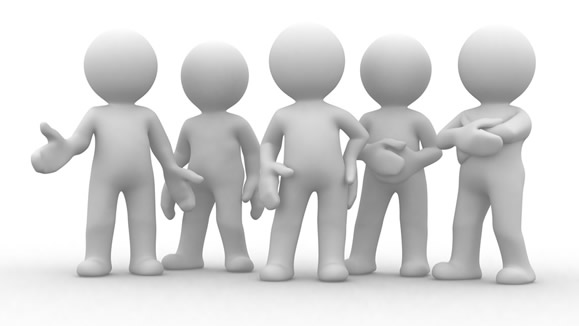
\includegraphics[width=\linewidth]{group1.jpg}
  \caption{Gruppen SAFE24 (www.gaia3d.co.uk/about/ redigerad)}
  \label{fig:group1}
\end{figure}


\end{abstracts}
%\end{abstractlongs}


% ---------------------------------------------------------------------- 


% The original template provides and abstractseparate environment, if your institution requires them to be separate. I think it's easier to print the abstract from the complete thesis by restricting printing to the relevant page.
% \begin{abstractseparate}
%   
% Thesis Abstract -----------------------------------------------------


%\begin{abstractslong}    %uncommenting this line, gives a different abstract heading

\begin{abstracts}        %this creates the heading for the abstract page
Mot slutet på kursen Inbyggda System och Signaler fick studenter som läser andra året, ett examinationsarbete i samarbete med Axis i Lund. De fick låna en avancerad och en kostsam IP-kamera, samt ett litet elektriskt kit med en mikroprocessor och några sensorer. Projektet inleddes med en föreläsning från två Axis-anställda som sedan klargjorde att examinationsuppgiften var att komma på ett problem och en lösning till det problemet. En grupp, SAFE24, bestod av Louay, Yurdaer, George och Benjamin som sedan tidigare studier under utbildningens gång var bekanta med varandra. Det fanns olika idéer i gruppen om vad problemet skulle vara. Efter några möten kom det fram ett problem i samhället. Lösningen byggde främst på de komponenter som gruppen fick, dock fanns det utrymme för att köpa ytterligare fler förutsatt att det inte översteg en viss budget.



\begin{figure}[h]
  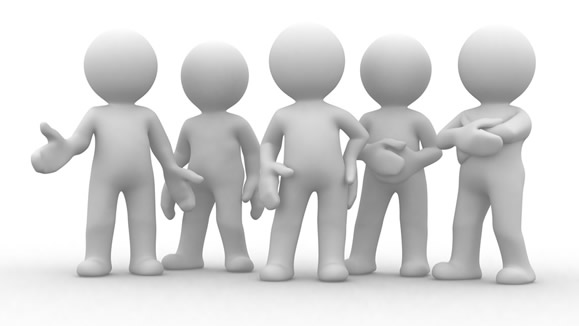
\includegraphics[width=\linewidth]{group1.jpg}
  \caption{Gruppen SAFE24 (www.gaia3d.co.uk/about/ redigerad)}
  \label{fig:group1}
\end{figure}


\end{abstracts}
%\end{abstractlongs}


% ---------------------------------------------------------------------- 

% \end{abstractseparate}


%: ----------------------- tie in front matter ------------------------

%\frontmatter
% Thesis Dedictation ---------------------------------------------------

\begin{dedication} %this creates the heading for the dedication page

Hittills har det inte varit några examinaationsprojekt på Datateknik-ingenjörsutbildningen, med sådana kompenenter som nämndes tidigare. Malmö Höskola har satsat mer på externa samarbeten, vilket gynnar skkola, studenter och även de externa samarbetsparterna.

Grupp SAFE24 vill tacka de ansvariga för programmet som ser till att sådant kan gå i verk och vill även tacka Axis från Lund som stödjer elever och skolverksamhet rent generellt.

\end{dedication}

% ----------------------------------------------------------------------

% Thesis Acknowledgements ------------------------------------------------


%\begin{acknowledgementslong} %uncommenting this line, gives a different acknowledgements heading
\begin{acknowledgements}      %this creates the heading for the acknowlegments

Mot slutet på kursen Inbyggda System & Signaler fick vi ett examinationsarbete i samarbete med Axis i Lund. Vi fick en avancerad och inte minst en dyr ip-kamera samt ett litet elektriskt kit med en mikroprocessor och några sensorer. Projektet inleddes med en intressant föreläsning från två Axis-anställda som sedan klargjorde att vår uppgift var att komma på ett problem och en lösning till det problemet. 
\end{acknowledgements}
%\end{acknowledgmentslong}

% ------------------------------------------------------------------------





%: ----------------------- contents ------------------------

\setcounter{secnumdepth}{3} % organisational level that receives a numbers
\setcounter{tocdepth}{3}    % print table of contents for level 3
\tableofcontents            % print the table of contents
% levels are: 0 - chapter, 1 - section, 2 - subsection, 3 - subsection


%: ----------------------- list of figures/tables ------------------------

%: ----------------------- glossary ------------------------

% Tie in external source file for definitions: /0_frontmatter/glossary.tex
% Glossary entries can also be defined in the main text. See glossary.tex
 
\newpage
\begin{multicols}{2} % \begin{multicols}{#columns}[header text][space]
\begin{footnotesize} % scriptsize(7) < footnotesize(8) < small (9) < normal (10) % target name for links to glossary\nomenclature{MLP}{Multilayerperceptron; a type of network that includes one layer of input nodes, a arbitrary count of hidden layers and a output layer of nodes} 
\printglossaries

\end{footnotesize}
\end{multicols}



%: --------------------------------------------------------------
%:                  MAIN DOCUMENT SECTION
% --------------------------------------------------------------

% the main text starts here with the introduction, 1st chapter,...
%\mainmatter

\renewcommand{\chaptername}{} % uncomment to print only "1" not "Chapter 1"

%: ----------------------- subdocuments ------------------------

% Parts of the thesis are included below. Rename the files as required.
% But take care that the paths match. You can also change the order of appearance by moving the include commands.

% this file is called up by thesis.tex
% content in this file will be fed into the main document

%: ----------------------- introduction file header -----------------------


\chapter{Inledning}

\setcounter{page}{1}
% the code below specifies where the figures are stored
\ifpdf
    \graphicspath{{1_introduction/figures/PNG/}{1_introduction/figures/PDF/}{1_introduction/figures/}}
\else
    \graphicspath{{1_introduction/figures/EPS/}{1_introduction/figures/}}
\fi

Mot slutet på kursen Inbyggda System och Signaler fick vi studenter på andra läsåret på Malmö Högskola ett examinationsarbete i samarbete med Axis i Lund. En avencerad IP-kamera, samt ett litet elektriskt kit med ett utvecklingskort och några sensorer användes till detta projekt. Projektet inleddes med en föreläsning från två Axis-anställda som klargjorde att examinationsuppgiften var att komma på ett problem samt en lösning till det. Vår grupp SAFE24 bestående av Louay, Yurdaer, George och Benjamin, kom på att vandalisering runt omkring busshållplatser var dålig för sammhället rent ekonomiskt och även rent socialt eftersom det skapade otrygghet. Vår lösning till problemet byggde främst på de komponenter som vi fick samt några andra som köptes in.
\begin{figure}[h]

  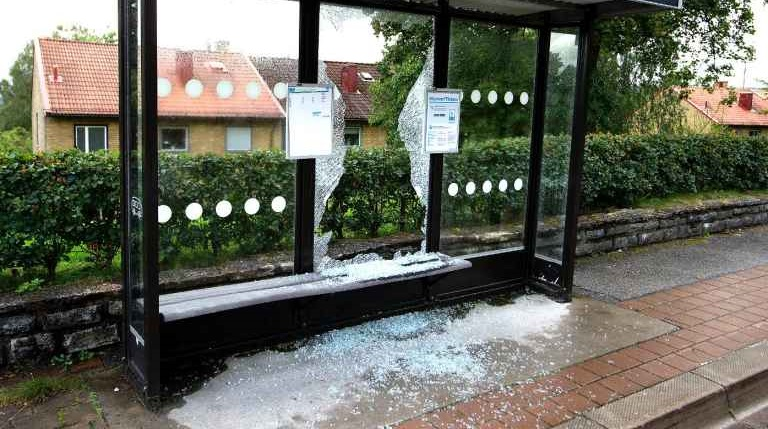
\includegraphics[width=\linewidth]{vandal.jpg}
  \caption{En vandaliserad hållplats i Borås. (www.bt.se/)}
  \label{fig:vandal}
\end{figure}

%: ----------------------- HELP: latex document organisation
% the commands below help you to subdivide and organise your thesis
%    \chapter{}       = level 1, top level
%    \section{}       = level 2
%    \subsection{}    = level 3
%    \subsubsection{} = level 4
% note that everything after the percentage sign is hidden from output

\newglossaryentry{ANN}{name={ANN},
description={Artificial Neural Network, a generic name for different machine learning models that mimic how learning is done in nature.}}

%\section{put section name here} % section headings are printed smaller than chapter names
% intro



%\subsection{Name your subsection} % subsection headings are again smaller than section names
% lead
%Different organised systems have different energy currencies. The machines that enable us to do science like sizzling electricity but at a controlled voltage. Earth's living beings are no different, except that they have developed another preference. They thrive on various chemicals. 

% dextran, starch, glycogen
%Most organisms use polymers of glucose units for energy storage and differ only slightly in the way they link together monomers to sometimes gigantic macromolecules. Dextran of bacteria is made from long chains of $\alpha$-1,6-linked glucose units. 

%: ----------------------- HELP: special characters
% above you can see how special characters are coded; e.g. $\alpha$
% below are the most frequently used codes:
%$\alpha$  $\beta$  $\gamma$  $\delta$

%$^{chars to be superscripted}$  OR $^x$ (for a single character)
%$_{chars to be suberscripted}$  OR $_x$

%>  $>$  greater,  <  $<$  less
%≥  $\ge$  greater than or equal, ≤  $\ge$  lesser than or equal
%~  $\sim$  similar to

%$^{\circ}$C   ° as in degree C
%±  \pm     plus/minus sign

%$\AA$     produces  Å (Angstrom)




% dextran, starch, glycogen continued
%Starch of plants and glycogen of animals consists of $\alpha$-1,4-glycosidic glucose polymers \cite{lastname07}. See figure \ref{largepotato} for a comparison of glucose polymer structure and chemistry. 

%Two references can be placed separated by a comma \cite{lastname07,name06}.

%: ----------------------- HELP: references
% References can be links to figures, tables, sections, or references.
% For figures, tables, and text you define the target of the link with \label{XYZ}. Then you call cross-link with the command \ref{XYZ}, as above
% Citations are bound in a very similar way with \cite{XYZ}. You store your references in a BibTex file with a programme like BibDesk.





%\figuremacro{largepotato}{A common glucose polymers}{The figure shows starch granules in potato cells, taken from \href{http://molecularexpressions.com/micro/gallery/burgersnfries/burgersnfries4.html}{Molecular Expressions}.}

%: ----------------------- HELP: adding figures with macros
% This template provides a very convenient way to add figures with minimal code.
% \figuremacro{1}{2}{3}{4} calls up a series of commands formating your image.
% 1 = name of the file without extension; PNG, JPEG is ok; GIF doesn't work
% 2 = title of the figure AND the name of the label for cross-linking
% 3 = caption text for the figure

%: ----------------------- HELP: www links
% You can also see above how, www links are placed
% \href{http://www.something.net}{link text}

%\figuremacroW{largepotato}{Title}{Caption}{0.8}
% variation of the above macro with a width setting
% \figuremacroW{1}{2}{3}{4}
% 1-3 as above
% 4 = size relative to text width which is 1; use this to reduce figures




%Insulin stimulates the following processes:

%\begin{itemize}
%\item muscle and fat cells remove glucose from the blood,
%\item cells breakdown glucose via glycolysis and the citrate cycle, storing its energy in the form of ATP,
%\item liver and muscle store glucose as glycogen as a short-term energy reserve,
%\item adipose tissue stores glucose as fat for long-term energy reserve, and
%\item cells use glucose for protein synthesis.
%\end{itemize}

%: ----------------------- HELP: lists
% This is how you generate lists in LaTeX.
% If you replace {itemize} by {enumerate} you get a numbered list.


 


%: ----------------------- HELP: tables
% Directly coding tables in latex is tiresome. See below.
% I would recommend using a converter macro that allows you to make the table in Excel and convert them into latex code which you can then paste into your doc.
% This is the link: http://www.softpedia.com/get/Office-tools/Other-Office-Tools/Excel2Latex.shtml
% It's a Excel template file containing a macro for the conversion.

%\begin{table}[htdp]
%\centering
%\begin{tabular}{ccc} % ccc means 3 columns, all centered; alternatives are l, r

%{\bf Gene} & {\bf GeneID} & {\bf Length} \\ 
% & denotes the end of a cell/column, \\ changes to next table row
%\hline % draws a line under the column headers

%human latexin & 1234 & 14.9 kbps \\
%mouse latexin & 2345 & 10.1 kbps \\
%rat latexin   & 3456 & 9.6 kbps \\
% Watch out. Every line must have 3 columns = 2x &. 
% Otherwise you will get an error.

%\end{tabular}
%\caption[title of table]{\textbf{title of table} - Overview of latexin genes.}
% You only need to write the title twice if you don't want it to appear in bold in the list of tables.
%\label{latexin_genes} % label for cross-links with \ref{latexin_genes}
%\end{table}



% There you go. You already know the most important things.


% ----------------------------------------------------------------------



	% background information
%% this file is called up by thesis.tex
% content in this file will be fed into the main document

\chapter{Aims of the project} % top level followed by section, subsection


% ----------------------- contents from here ------------------------

\section{Final aim}

\section{Preliminary aims}


% ---------------------------------------------------------------------------
% ----------------------- end of thesis sub-document ------------------------
% ---------------------------------------------------------------------------						% aims of the project
% this file is called up by thesis.tex
% content in this file will be fed into the main document

%: ----------------------- name of chapter  -------------------------
\chapter{Teori} % top level followed by section, subsection
\label{teori}

%: ----------------------- paths to graphics ------------------------
\ifpdf
    \graphicspath{{3_theory/figures/PNG/}{3/figures/PDF/}{3/figures/}}
\else
    \graphicspath{{3_theory/figures/EPS/}{3/figures/}}
\fi

\graphicspath{{3_theory/figures/}{3/figures/}}

%: ----------------------- contents from here ------------------------

\section{Problemlösning}

En busshållplats som är övervakad dygnet runt är en ineffektiv lösning. Övervakningen ska ske i samband med att specifika villkor är uppfyllda. Därför är glasen monterade med en varsin ljudsensor för att registrera antingen hårda slag mot glasytan eller även när glasen krossas. Dessa två händelser utgör ett huvudvilkor för att systemet ska aktveras. Om inget villkor är uppfyllt så kommer systemet att vara i ett passivt tillstånd och enbart lyssna på förändringar. Utöver det ska det finnas en PIR-sensor som detekterar rörelser inne i hållplatsen och med det tända en stor lampa. Lampan tänds för att ge en känsla av trygghet för dem som väntar inne i hållplatsen, men även för att uppmärksamma bussarna och andra i omgivningen om att någon rör sig i hållplatsen. \\

I mitten av vägen ska det finnas en IP-kamera som vid tidigare nämda vilkor aktiveras och först riktar sig mot den ljudsensor som har registrerat en händelse för att filma i den riktningen ett antal sekunder innan den forsätter filmandet medan den roterar 360 grader tillbaka till den första punkten. Där filmar den ytterligare några sekunder till i samma riktning. Därefter slutar kameran att filma och återgår till ett passivt läge.

\begin{figure}[h]
  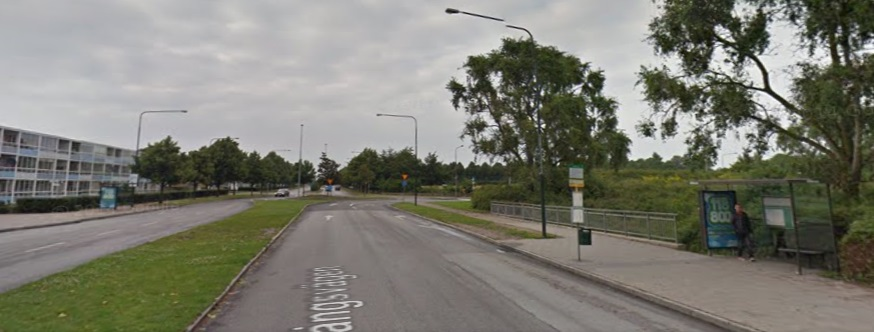
\includegraphics[width=\linewidth]{lind.jpg}
  \caption{En obevakad hållplats i Malmös stadsdel Lindängen. (Google Maps: Lindängen - Malmö)}
  \label{fig:lind}
\end{figure}




% ---------------------------------------------------------------------------
%: ----------------------- end of thesis sub-document ------------------------
% ---------------------------------------------------------------------------

			
\include{4/XYZ}	
\include{5/XYZ}



% this file is called up by thesis.tex



\chapter{Material \& Metoder} % top level followed by section, subsection
\label{ch:metoder}

% ----------------------- paths to graphics ------------------------

% change according to folder and file names
\ifpdf
    \graphicspath{{8/figures/PNG/}{8_materials_and_methods/figures/PDF/}{8_materials_and_methods/figures/}}
\else
    \graphicspath{{8/figures/EPS/}{8_materials_and_methods/figures/}}
\fi

% ----------------------- contents from here ------------------------

\section{Material}
I vår lösning använde vi oss av ett utvecklingskort ESP8266 med ett inbyggt Wifi som var nödvändig för att kunna kommunicera med det nätverk som kameran var uppkopplad till.

Kameran är av modellen Q6128-E Network Camera med möjlighet till internetuppkoppling. Upplösningen som används är 3840x2860. Ett suffix med datum och tidsinformation läggs till i filnamnet för inspelningen.

En PIR-sensor från Adafruit användes som rörelsedetektor för att tända lampan i hållplatsen.

Som nämt tidigare i rapporten använde vi oss av en ljudsensor som var monterad mot en glasyta. Vid besök hos en elektrokit-grossist kunde vi inte få tag på någon användbar trycksensor som var tillräckligt känslig för att ersätta ljudsensorn. Under demo-dagen fick vi frågan om vi hade tänkt på en Piezo-sensor, som är en typ av en tryck-sensor. Efter fakta-sökning fann vi att en Piezo-sensor hade varit ett bättre alternativ än ljudsensorn.

För att kunna identifiera att någon har utfört vandalisering måste systemet lagra bilder/inspelningar på en server. En FTP-server användes. FTP-servern och IP-kameran låg i samma subnät.\\

Information om FTP-servern:

\begin{itemize}
\item IP adress : 192.168.0.106

\item Port nummer : 21

\item Användarnamn : ”FTP-User”

\item Lösenord : ”Safe24”

\end{itemize}

\begin{figure}[h]

  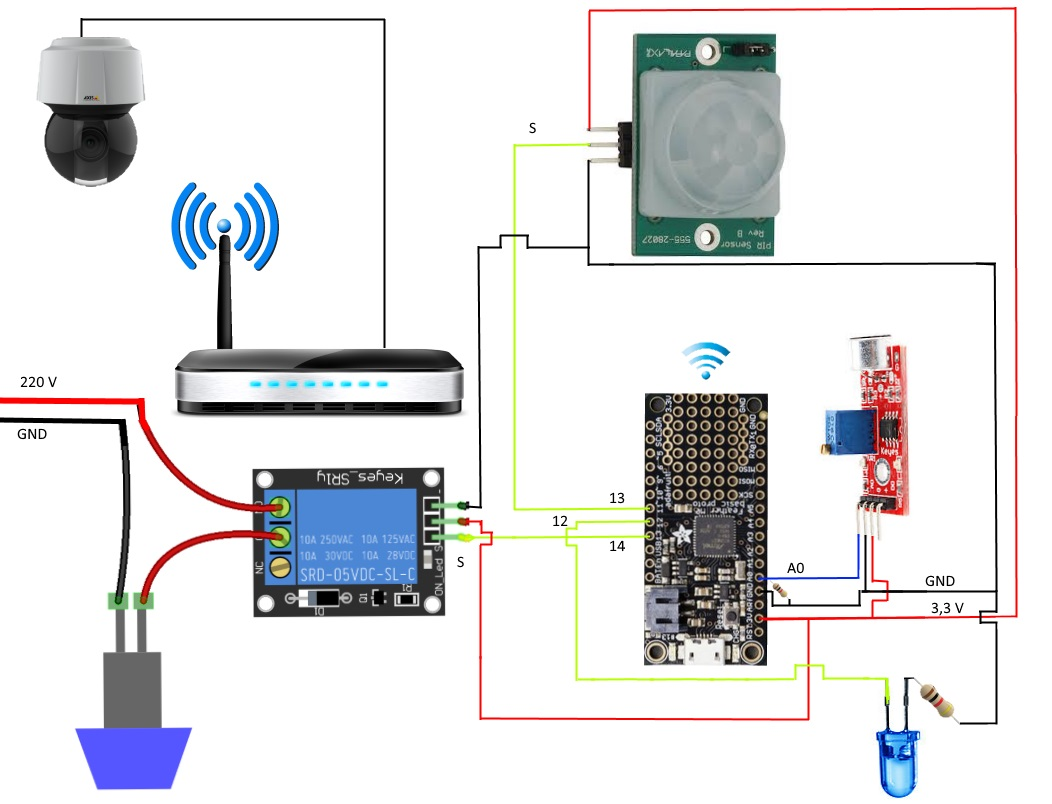
\includegraphics[width=\linewidth]{connections.jpg}
  \caption{Alla komponenter kopplade med varandra.)}
  \label{fig:connections}
\end{figure}
\clearpage



\section{Metoder} 
Om PIR-sensorn detekterar någon rörelse då skall lampan tändas en viss tid och sedan släckas. Om lampan är tänd och PIR-sensorn detekterar ny rörelse då fortsätter lampan vara tänd. För att lyckas med PIR-sensorn fick vi med hjälp av några delays och räknare räkna in hur många gånger som signalen var hög eller låg. Efter flera tester och försök kom vi fram till att det behövdes minst sju rundor med en runda på 0,5 sekunder. Anledningen till detta var att när det inte fanns någon rörelse så gav PIR-sensorn utslag med några ettor samt några nollor. Då det fanns rörelse gav den utslag på bara ettor.\\

 Ljud-sensorn är också igång hela tiden. Om ljudsensorn detekterar ett ljud som är över gränsvärdet skall den viktiga processen börja. På grund av brist på glas och utrymme för oss att göra testförsök med att ta sönder glas använde vi istället plast. Plasten skulle föreställa glaset i en busshållplats. Vi kom överens om att sätta tröskelvärdet till 75 utav max 1024 som analoga ingången kunde läsa. Över denna gräns indikerades att glas hade gått sönder.\\

IP-kameran var installerad i mitten av vägen så att den kan rotera fritt eftersom vandaliseringen kan ske på avstånd från hållplatsen. Den var ansluten via ethernet och vi styrde den med hjälp av http-kommando som utvecklingskortet skickade iväg. Vi fick kamerans http-API (VAPIX) från Axis. Inne i kameran skapade vi tre events ActionPTZStation1, ActionRecord, ActionPTZHome.

ActionPTZStation1: När virtuell port 8 aktiveras så riktas kameran mot en bestämd position som  heter "plats1" (busshållplatsen).

ActionRecord: När virtuell port 9 aktiveras så börjar kameran videoinspelningen. Efter avslutad inspelning skickas klippet till FTP-servern.

ActionPTZHome: När virtuell port 10 aktiveras så riktas kameran mot en bestämd position som heter Safe24 och som motsvarar start och slutpositionen för kameran.\\

Det finns totalt tre tasks i systemet som exekveras parallellt för att kunna låta processorn
jobba med flera saker samtidigt. Biblioteket som används att schemalägga tasks är skapat av Nicholas Wiersma och heter ESP8266Scheduler.

Två av de tre tasksen (pirsensorn och ljudsensorn) agerar som inputs till systemet. Den tredje tasken (WifiTask) kontrollerar om det finns en wifi-anslutning, om anslutningen är nere försöker den återansluta till wifi.


 








\clearpage
\section{Systembeskrivning}
Vi har nämt tidigare i rapporten att vårt kamerasystem skall befinna sig i ett passivt läge så länge inget villkor är uppfyllt. Om ett villkor är uppfyllt då aktiveras två virtuella portar i kameran. Den ena riktar kameran mot busshållplatsen (port 8) och den andra (port 9) gör att kameran börjar filma. Då filmar kameran i fem sekunder och sedan filmar den runt omkring medan den vrider sig horisontellt. Efter ett varv riktas kameran mot busshållplatsen igen och det görs genom att aktivera virtuell port 9. Kameran ska forsätta filma några sekunder till och efter det ska den riktas mot sitt standardläge dvs ActionPTZHome. Den totala videolängden är 40 sekunder och filmen skickas till FTP-servern. Ifall ljudsensor detekterar ett annat ljud som är över gränsen inom 40 sekunder då ska processen börja från början dvs kameran riktas tillbaka mot bushållplatsen osv.\\
 Samtidigt som utvecklingskortet väntar på utslag från ljudsensorn, väntar den på utslag från PIR-sensorn. När någon rör sig inne i hållplatsen ser utvecklingskortet till att en lampa tänds och släcks en viss tidsperiod som hela tiden förlängs vid nya rörelser. I det fall där kamerasystemet aktiveras, tar kamerasystemet över PIR-sensorn och låter lampan att blinka tills kamerasystemet är tillbaka till sitt passiva läge.

\section{Arbetsuppgifter}
Gruppen arbetade både tillsammans och även enskilt så att var och en av gruppmedlemmarna kunde bidra med något. Benjamin var delaktig i arbetet med flödesdiagram, tasks, hjälp med byggandet av busshållplats och även testfall. Yurdaer arbetade med wifi-kodning av ESP:n, kamera-kommandon, ftp-servern och i rapporten skrev han om sina delar samt om etiska aspekter. Georges bidrag var med struktur av kod, API, manual, testfall, FTP-servern och en del rapportskrivning. Han bidrog även med upprättande av en Latex-mall för rapporten. Louay arbetade med sensorernas kodning, ihopkoppling av alla komponenter, förslag till router-lösning, byggandet av en hållplats och kontinuerlig testning av alla kopplingar. 
% ---------------------------------------------------------------------------
%: ----------------------- end of thesis sub-document ------------------------
% ---------------------------------------------------------------------------



 



               % description of lab methods results
% this file is called up by thesis.tex
% content in this file will be fed into the main document


%: ----------------------- name of chapter  -------------------------
\chapter{Resultat} % top level followed by section, subsection
\label{ch:resultat}

%: ----------------------- paths to graphics ------------------------

% change according to folder and file names
\ifpdf
    \graphicspath{{6/figures/PNG/}{6/figures/PDF/}{6/figures/}}
\else
    \graphicspath{{6/figures/EPS/}{6/figures/}}
\fi

%: ----------------------- contents from here ------------------------


\section{Testfall}

Under testfasen användes det webbaserade programmet testrail. Fördelen med det var att flera personer kunde lägga till och redigera testfallen samt att vi fick en grafisk överblick över vilka testfall som har passerat respektive fallerat. 
Testfallen skrevs på så sätt att de skulle validera systemlösningen vilket gick ut på att kontrollera kamerans bestämda rörlighet, sensorernas känslighet, kommunikationen mellan esp8266 och kameran, kommunikationen mellan kameran och ftp-servern samt att testa kamerans anslutning till wifi nätverket.
Vi testade schemaläggningen genom att skriva ut ett visst ord i slutet av varje task, och vänta på att se det ordet utskrivet. När vi startade programmet såg vi att vissa task kördes flera gånger innan den hoppade till nästa task, dock kördes alla task i ordning. 
Resultaten från samtliga testfall överensstämde med det förväntade resultatet. Som en följd av detta passerade alla tester och inga justeringar av systemlösningen var nödvändiga. Med andra ord har systemlösningen validerats att den löser problemet genom testningen.



% ---------------------------------------------------------------------------
%: ----------------------- end of thesis sub-document ------------------------
% ---------------------------------------------------------------------------


% this file is called up by thesis.tex
% content in this file will be fed into the main document

\chapter{Diskussion \& Framtid} % top level followed by section, subsection
\label{ch:diskussion}

% ----------------------- paths to graphics ------------------------

% change according to folder and file names
\ifpdf
    \graphicspath{{7/figures/PNG/}{7/figures/PDF/}{7/figures/}}
\else
    \graphicspath{{7/figures/EPS/}{7/figures/}}
\fi


% ----------------------- contents from here ------------------------



\section{Diskussion}
\subsection{Lagar och Etsika Aspekter}
I Sverige det finns regler som gäller för kameraövervakning. Kameraövervakningslagen (2013:460) omfattar dels övervakningskameror dels tekniska anordningar för att behandla eller bevara bilder och andra tekniska anordningar för avlyssning eller upptagning av ljud som används i samband med övervakningskameror \cite{lansstyrelsen}. 
Enligt huvudregeln är att tillstånd krävs om:

\begin{itemize}
\item kameran riktas mot "en plats dit allmänheten har tillträde"

\item utrustningen kan användas för personbevakning och

\item kameran är uppsatt utan att manövreras på platsen
\end{itemize}
I definitionen ”allmänheten har tillträde” tar man ingen hänsyn till om det handlar om privat eller allmän mark, utan alla platser dit allmänheten någon gång har tillträde omfattats av lagen om allmän övervakning. Busshållplatser och gatorna räknas som allmänt platser enligt definitionen av allmänt plats.  Det här ställer vissa krav på den som installerar och/eller äger det systemet som vi har skapat under den examinations projekt. Man måste se till att lagar och regler följs dvs man måste göra en ansökan om tillstånd till allmän kameraövervakning. 
Kameraövervakning är en metod som används för att minska brottsligheten. Effekterna varierar beroende på hur man arbetar med kamerorna. Andra sidan är kameraövervakning alltid känsligt utifrån ett integritetsperspektiv. Det som är människor oroliga för när det gäller övervakningskameror är att integritet av människors privata liv.  Det är människors privatliv som människor har rätt beskydda. En ingenjör bör respektera detta som alla andra människor. Ingenjörer har ansvar att verka för att tekniken används för samhällets och mänsklighetens bästa enligt hederskodexen för Sveriges ingenjörer \cite{sverige}. Vi använder kameraövervakningen med ett syfte som är att bekämpa brott. 




% ---------------------------------------------------------------------------
% ----------------------- end of thesis sub-document ------------------------
% ---------------------------------------------------------------------------      			    % discussion of




% --------------------------------------------------------------
%:                  BACK MATTER: appendices, refs,..
% --------------------------------------------------------------

% the back matter: appendix and references close the thesis


%: ----------------------- bibliography ------------------------

% The section below defines how references are listed and formatted
% The default below is 2 columns, small font, complete author names.
% Entries are also linked back to the page number in the text and to external URL if provided in the BibTex file.

% PhDbiblio-url2 = names small caps, title bold & hyperlinked, link to page 
\begin{multicols}{2} % \begin{multicols}{ # columns}[ header text][ space]
\begin{tiny} % tiny(5) < scriptsize(7) < footnotesize(8) < small (9)

%\bibliographystyle{Latex/Classes/PhDbiblio-url2} % Title is link if provided
%\renewcommand{\bibname}{References} % changes the header; default: Bibliography

%\bibliography{9_backmatter/references} % adjust this to fit your BibTex file

\end{tiny}
\end{multicols}

% --------------------------------------------------------------
% Various bibliography styles exit. Replace above style as desired.

% in-text refs: (1) (1; 2)
% ref list: alphabetical; author(s) in small caps; initials last name; page(s)
%\bibliographystyle{Latex/Classes/PhDbiblio-case} % title forced lower case
%\bibliographystyle{Latex/Classes/PhDbiblio-bold} % title as in bibtex but bold
%\bibliographystyle{Latex/Classes/PhDbiblio-url} % bold + www link if provided

%\bibliographystyle{Latex/Classes/jmb} % calls style file jmb.bst
% in-text refs: author (year) without brackets
% ref list: alphabetical; author(s) in normal font; last name, initials; page(s)

%\bibliographystyle{plainnat} % calls style file plainnat.bst
% in-text refs: author (year) without brackets
% (this works with package natbib)


% --------------------------------------------------------------

% according to Dresden med fac summary has to be at the end
%
% Thesis Abstract -----------------------------------------------------


%\begin{abstractslong}    %uncommenting this line, gives a different abstract heading

\begin{abstracts}        %this creates the heading for the abstract page
Mot slutet på kursen Inbyggda System och Signaler fick studenter som läser andra året, ett examinationsarbete i samarbete med Axis i Lund. De fick låna en avancerad och en kostsam IP-kamera, samt ett litet elektriskt kit med en mikroprocessor och några sensorer. Projektet inleddes med en föreläsning från två Axis-anställda som sedan klargjorde att examinationsuppgiften var att komma på ett problem och en lösning till det problemet. En grupp, SAFE24, bestod av Louay, Yurdaer, George och Benjamin som sedan tidigare studier under utbildningens gång var bekanta med varandra. Det fanns olika idéer i gruppen om vad problemet skulle vara. Efter några möten kom det fram ett problem i samhället. Lösningen byggde främst på de komponenter som gruppen fick, dock fanns det utrymme för att köpa ytterligare fler förutsatt att det inte översteg en viss budget.



\begin{figure}[h]
  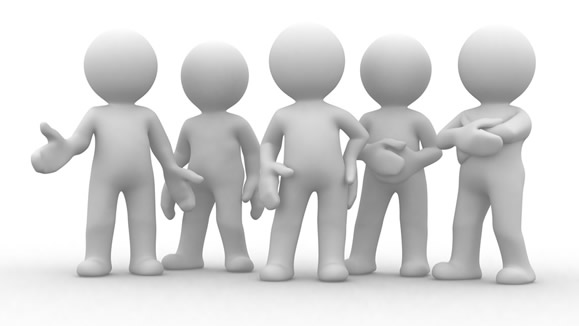
\includegraphics[width=\linewidth]{group1.jpg}
  \caption{Gruppen SAFE24 (www.gaia3d.co.uk/about/ redigerad)}
  \label{fig:group1}
\end{figure}


\end{abstracts}
%\end{abstractlongs}


% ---------------------------------------------------------------------- 


%: Declaration of originality
%
% Thesis statement of originality -------------------------------------

% Depending on the regulations of your faculty you may need a declaration like the one below. This specific one is from the medical faculty of the university of Dresden.

\begin{declaration}        %this creates the heading for the declaration page

I herewith declare that I have produced this paper without the prohibited assistance of third parties and without making use of aids other than those specified; notions taken over directly or indirectly from other sources have been identified as such. This paper has not previously been presented in identical or similar form to any other Swedish or foreign examination board.

The thesis work was conducted from 2012-09-01 to 2013-05-XX under the supervision of Patrik Edén at the Department of astronomy and theoretical physics.

\vspace{10mm}

MALMÖ,


\end{declaration}


% ----------------------------------------------------------------------



\begin{thebibliography}{50}


\bibitem{haykin} S. Haykin, Neural Networks and Learning Machines (Pearson Prentice Hall, 3rd edition, 2009)


\bibitem{mit} K.O. Stanley and R. Miikkulainen, Evolving Neural Networks through Augmenting Topologies, Evolutionary Computation \textbf{10}, 99-127 (2002)

\bibitem{DavidJ} D.J. Montana and L. Davis, Training Feedforward Neural Networks Using Genetic Algorithms, In Proceedings of the International Joint Conference on Artificial Intelligence, pp. 762-767 (1989)

\bibitem{pima}  J.W. Smith, J.E. Everhart, W.C. Dickson, W.C. Knowler and  
R.S. Johannes, Using the ADAP learning algorithm to forecast the onset of 
diabetes mellitus, In Proceedings of the Symposium on Computer 
Applications and Medical Care, pp. 261-265 (1988)


\bibitem{neuroph} http://neuroph.sourceforge.net/

\end{thebibliography}
\end{document}
